\section{Experiments}\label{sec:exp}

\subsection{Setup, protocol, and scope}\label{sec:exp-setup}

\paragraph{Models.}
GPT-2 (124M; 12 layers, 12 heads, multi-head attention, 1{,}024-token
native window)~\cite{radford2019gpt2} and
Qwen2.5-0.5B-Instruct (24 layers, 14 query / 2 KV heads, grouped-query
attention, 32K native window)~\cite{qwen2025}. The pair spans the two
attention architectures in current use and deliberately avoids any
position-encoding surgery: every context we evaluate is native to the
model, which removes the context-extension confound of our earlier
manuscript (which extended a 4K-native model to 128K with an undocumented
interpolation factor).

\paragraph{Harness.}
All methods run in one engine: chunked prefill and greedy decode with
chunk size 64, eager attention for exact score extraction, per-layer
causal masking over retained entries (Section~\ref{sec:method}), explicit
absolute position ids, and cache surgery by index selection. Compression
runs after every chunk, invoking the projector of
Theorem~\ref{thm:exact} and asserting the contract; every configuration
also writes a per-step accounting record (retained entries, nominal
budget, auxiliary bytes, timing). Perplexity uses teacher forcing on
WikiText-2 test \cite{merity2016wikitext}: 32 non-overlapping
1{,}024-token windows for GPT-2 and 10 non-overlapping 2{,}048-token
windows for Qwen2.5-0.5B; each position's prediction sees exactly the
cache state a deployed system would have after compressing the prefix at
the last chunk boundary.

\paragraph{Matched-entry baselines.}
All baselines share the projector, the floors, and the caps of
Section~\ref{sec:method}: \textbf{StreamingLLM} (sinks plus a window
grown to the budget, no scores)~\cite{xiao2024streamingllm};
\textbf{H2O} (cumulative scores, $\gamma=1$, uniform weights)
\cite{zhang2023h2o}; \textbf{PyramidKV} (cumulative scores, static
bottom-heavy pyramid weights)~\cite{cai2024pyramidkv};
\textbf{Reverse-pyramid} (the mirrored control, testing whether direction
of the static prior matters); and \sage{} with its ablations
(no-decay $\gamma=1$; uniform-budget $\tau=0$; no-sink; no-recent).
Every method holds the \emph{same} retained-entry count at every step of
every run; auxiliary memory is reported separately
(Table~\ref{tab:main}). This is the protocol correction our earlier
manuscript lacked: comparisons there mixed nominal budgets with different
actual occupancies across methods.

\paragraph{Scope, stated plainly.}
The study runs on a 2-core CPU: models to $0.5$B parameters, contexts to
4{,}096 tokens, $\sim$61 tokens/s prefill on the Qwen model. We do not
measure GPU throughput, batching effects, or multi-GB-scale behaviour,
and we make no claims about them; the artifact includes a GPU replication
protocol (identical code paths, larger models and contexts) for groups
with the hardware. What the scale does support---and what this section
reports---is correctness of the memory contract under deployment
conditions, quality--memory trade-offs, mechanism attributions via
matched-entry ablations, and failure-mode diagnostics that do not depend
on scale.

\subsection{RQ1: Does the contract hold?}\label{sec:exp-compliance}

\begin{table}[t]
\centering\small
\caption{Budget compliance and per-chunk overhead. The original
entropy-exponent formula of our earlier manuscript is evaluated in
simulation over $2{,}048$ steps with drifting dispersion signals; the
projection is evaluated both in the same simulation and deployed inside
every experimental run (accounting logs; mean over all logged
configurations). Violations count steps where the realised cache exceeded
the advertised contract.}
\label{tab:compliance}
\begin{tabular*}{\columnwidth}{@{\extracolsep{\fill}} l c c c}
\toprule
Setting & Violations & Mean excess & Max excess \\
\midrule
Original formula (simulation) & 97.4\% & +4.2\% & +10.6\% \\
Corrected projection (simulation) & 0.0\% & 0.0\% & 0.0\% \\
\midrule
SAGE v2 (GPT-2, deployed) & 0 & 2.5\,ms & 1.9\,ms \\
H2O (GPT-2, deployed) & 0 & 3.3\,ms & 1.5\,ms \\
SAGE v2 (Qwen, deployed) & 0 & 6.5\,ms & 3.1\,ms \\
H2O (Qwen, deployed) & 0 & 8.7\,ms & 2.8\,ms \\
\bottomrule
\end{tabular*}
\end{table}

Table~\ref{tab:compliance} answers directly. The uncorrected formula
violates the contract in $97.4\%$ of simulated steps with a mean overshoot
of $+4.2\%$ and a maximum of $+10.6\%$ (Figure~\ref{fig:budget}); the
overshoot is the Jensen gap of Section~\ref{sec:intro} and it persists
under the formula's own lower clip. The corrected projection incurs zero
violations---in simulation, across $19{,}980$ randomised stress
instances, and deployed in every run of this paper
($3{,}840$ compression steps across all reported configurations, each
carrying a live assertion). The overhead of correctness is modest:
scoring plus projection plus eviction together add $2.5$--$9.6$\,ms per
64-token chunk on the two-core CPU, against $200$--$500$\,ms of forward
time per chunk.

\begin{figure}[t]
\centering
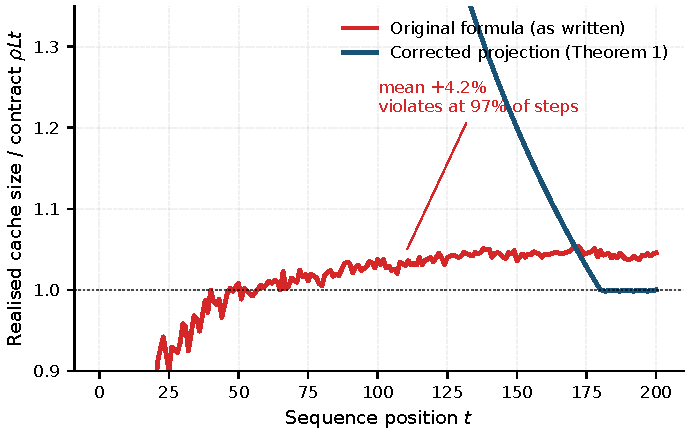
\includegraphics[width=0.78\columnwidth]{fig_budget.pdf}
\caption{Realised cache size relative to the proportional contract
$\rho Lt$ over the first 200 steps of the simulation. The original
entropy-exponent formula (red) drifts above the contract at nearly every
step; the corrected projection (blue) sits exactly on the contract after
the explicit warmup allowance of Eq.~\eqref{eq:contract}.}
\label{fig:budget}
\end{figure}

\subsection{RQ2: Language modelling quality at matched entries}

\begin{table}[t]
\centering\small
\caption{WikiText-2 perplexity at $\rho=0.2$ under the matched-entry
protocol (mean over 32$\times$1{,}024 tokens for GPT-2; 10$\times$2{,}048
for Qwen2.5-0.5B). Every compressed method holds the same retained-entry
count at every step. Aux.\ is measured auxiliary memory (scores, indices,
budget state; MB) at the end of a sequence, GPT-2 / Qwen.}
\label{tab:main}
\begin{tabular*}{\columnwidth}{@{\extracolsep{\fill}} l c c c}
\toprule
Method & GPT-2 PPL & Qwen PPL & Aux.\ (MB) \\
\midrule
Full cache (reference) & 32.41 & 13.37 & 0.10 / 0.39 \\
StreamingLLM (sinks + window) & 59.92 & 17.65 & 0.02 / 0.08 \\
H2O (cumulative, uniform budget) & 49.63 & 16.78 & 0.01 / 0.08 \\
PyramidKV (cumulative, static pyramid) & 50.77 & 18.27 & 0.03 / 0.08 \\
Reverse pyramid (control) & 69.03 & 16.71 & 0.02 / 0.08 \\
SAGE v2 (decay + entropy budget) & 49.80 & 17.02 & 0.02 / 0.08 \\
SAGE v2 w/o decay ($\gamma{=}1$) & 47.58 & 17.43 & 0.02 / 0.08 \\
SAGE v2 w/ uniform budget ($\tau{=}0$) & 54.00 & 16.40 & 0.02 / 0.08 \\
\bottomrule
\end{tabular*}
\end{table}

\begin{figure}[t]
\centering
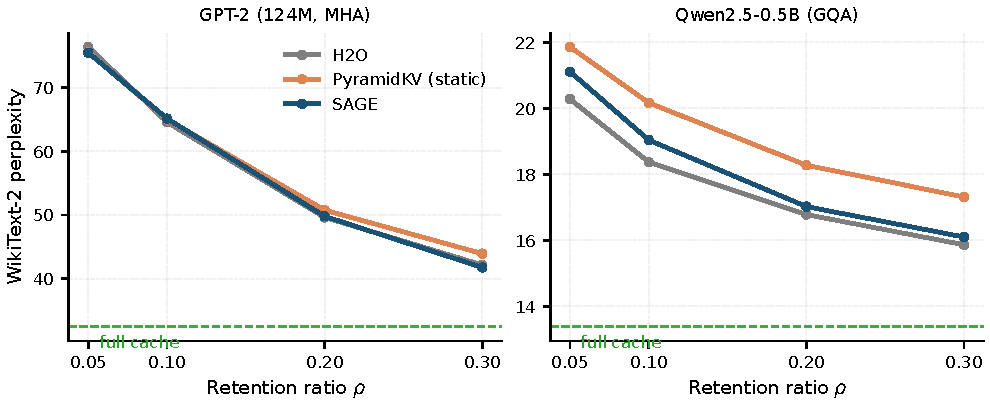
\includegraphics[width=\columnwidth]{fig_ppl_curve.pdf}
\caption{Perplexity versus retention ratio $\rho\in\{0.05,0.1,0.2,0.3\}$
at matched entries. On GPT-2 (left), dispersion-adaptive \sage{} tracks
or beats H2O at every $\rho$ and is best at $\rho=0.3$; the static
pyramid is uniformly worse than uniform allocation on this model. On
Qwen2.5-0.5B (right), \sage{} dominates the static pyramid at every
$\rho$ but is matched by uniform-budget variants, showing the value of
adaptivity is architecture-dependent.}
\label{fig:pplcurve}
\end{figure}

Table~\ref{tab:main} and Figure~\ref{fig:pplcurve} report the main
perplexity comparison; four findings stand out, two favourable and two
sobering. \emph{Favourable:} (1) allocation \emph{direction} matters
enormously---the reverse-pyramid control is catastrophic on GPT-2 (PPL
69.03, $39\%$ worse than uniform H2O) while remaining benign on Qwen
(16.71), i.e., a wrong static prior is model-dependent poison;
(2) dispersion-adaptive budgets beat the static pyramid on both
architectures (GPT-2: 49.80 vs.\ 50.77 at $\rho=0.2$ with default
$\gamma$, and 47.58 vs.\ 50.78 without decay; Qwen: 17.02 vs.\ 18.27),
and beat uniform budgets clearly on GPT-2 (47.58 vs.\ 49.63). \emph{Sobering:}
(3) on Qwen2.5-0.5B the strongest single setting is \sage{} with uniform
budgets (16.40), i.e., adaptivity did not pay on this model at this
scale---although the adaptive variant still dominates the static prior by
1.25 points; (4) default-rate decay costs perplexity on both models
(GPT-2: 49.80 vs.\ 47.58 without decay), a trade-off RQ4 quantifies and
RQ5 prices against retrieval. Auxiliary memory is small for every method
($\le0.39$\,MB at these scales, Table~\ref{tab:main}), but we report it
because at longer contexts it scales linearly with retained entries and
belongs in any honest budget.

\subsection{RQ3: What does the allocator actually do?}
\label{sec:exp-alloc}

\begin{figure}[t]
\centering
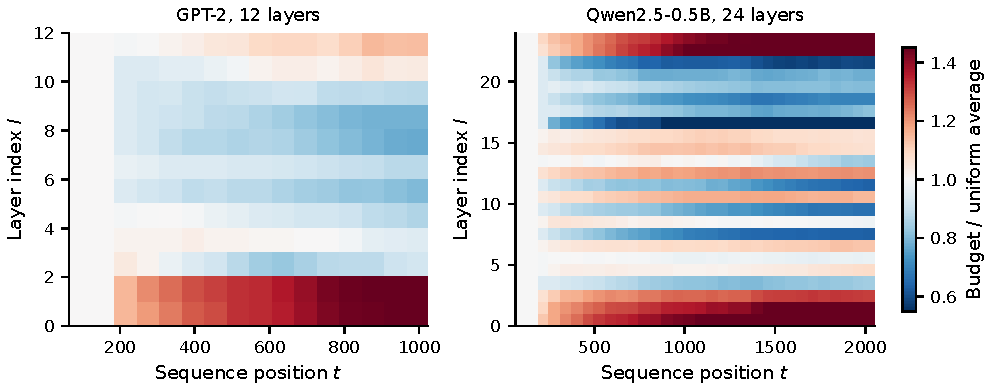
\includegraphics[width=\columnwidth]{fig_alloc.pdf}
\caption{Per-layer budgets over time (relative to the uniform average)
under \sage{} at $\rho=0.2$, from the accounting traces. The allocation
follows measured dispersion online, differs strongly between the two
architectures, and is not a fixed pyramid.}
\label{fig:alloc}
\end{figure}

\begin{figure}[t]
\centering
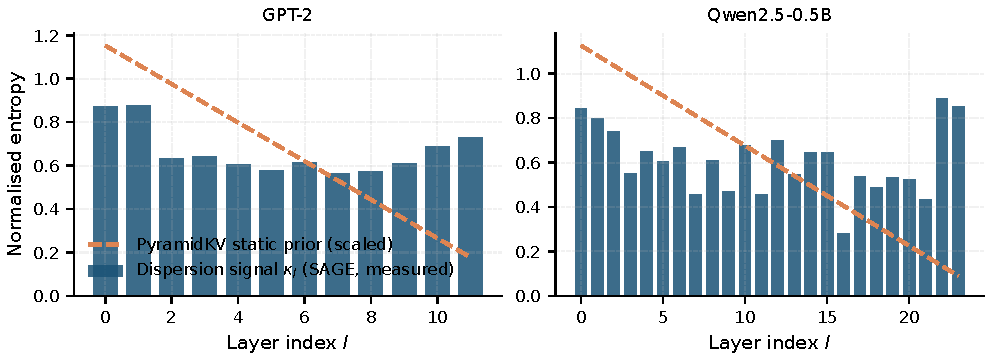
\includegraphics[width=\columnwidth]{fig_kappa.pdf}
\caption{Measured dispersion signal $\kappa_l$ at the end of a sequence
(bars) against the static PyramidKV prior rescaled to the same mean
(dashed). GPT-2's profile is non-monotone in depth---no static pyramid
can match it; Qwen2.5-0.5B's profile rises mid-network then falls.}
\label{fig:kappa}
\end{figure}

Figures~\ref{fig:alloc} and~\ref{fig:kappa} open the allocator's black
box. On GPT-2 the measured dispersion profile is non-monotone in depth,
so the static bottom-heavy pyramid---whatever its provenance on other
families---\emph{cannot} fit it, explaining the uniform-allocation
advantage on that model (Table~\ref{tab:main}) and the reverse control's
catastrophe. On Qwen2.5-0.5B the profile rises through the middle of the
network before falling in the last third; the adaptive weights track it
online through the EMA-smoothed entropy signal, and the resulting
allocation (Figure~\ref{fig:alloc}, right) is bottom-heavy early in the
sequence and mid-heavy later. These traces are the direct empirical case
for measuring dispersion rather than assuming a profile: the two
architectures want visibly different allocations, and neither matches a
fixed prior.

\subsection{RQ4: Sensitivity---the decay trade-off and the exponent}
\label{sec:exp-sens}

\begin{table}[t]
\centering\small
\caption{Ablations and sensitivity on GPT-2 at $\rho=0.2$ (WikiText-2).
Ablation rows use the full 32-sequence set; sensitivity rows use a
16-sequence subset, hence the small offset between the two $\gamma{=}1$
rows. The no-sink ablation removes structural sink protection, keeping
everything else identical.}
\label{tab:sens}
\begin{tabular*}{0.86\columnwidth}{@{\extracolsep{\fill}} l c}
\toprule
Configuration & PPL \\
\midrule
SAGE v2 (default $\gamma{=}0.995$, $\tau{=}1.5$) & 49.80 \\
\;w/o decay ($\gamma{=}1$) & 47.58 \\
\;w/ uniform budget ($\tau{=}0$) & 54.00 \\
\;w/o sink protection & 4079.01 \\
\;w/o recent window & 55.62 \\
\midrule
Decay $\gamma{=}0.98$ & 54.50 \\
Decay $\gamma{=}0.99$ & 53.39 \\
Decay $\gamma{=}0.999$ & 46.90 \\
Decay $\gamma{=}1.0$ & 46.89 \\
Decay $\gamma{=}1.0$ (no decay) & 47.58 \\
Exponent $\tau{=}0.5$ & 51.40 \\
Exponent $\tau{=}1.0$ & 50.19 \\
Exponent $\tau{=}1.5$ & 49.80 \\
Exponent $\tau{=}2.0$ & 48.58 \\
\bottomrule
\end{tabular*}
\end{table}

\begin{figure}[t]
\centering
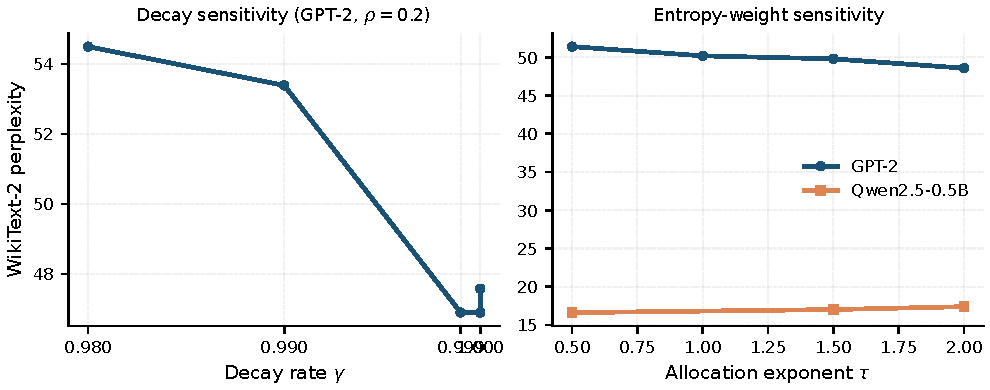
\includegraphics[width=\columnwidth]{fig_sens.pdf}
\caption{Left: perplexity versus decay rate $\gamma$ on GPT-2---language
modelling prefers slow or no decay. Right: perplexity versus exponent
$\tau$ on both models---GPT-2 prefers stronger dispersion weighting,
Qwen2.5-0.5B milder, consistent with the different dispersion profiles
of Figure~\ref{fig:kappa}.}
\label{fig:sens}
\end{figure}

Table~\ref{tab:sens} and Figure~\ref{fig:sens} quantify the two
mechanism dials. \emph{Decay} $\gamma$: perplexity improves monotonically
as decay weakens (54.50 at $\gamma=0.98$, 46.90 at $\gamma=0.999$, 46.89
at $\gamma=1$)---stationary WikiText text rewards long memory, exactly as
Proposition~\ref{prop:staleness}'s converse predicts. \emph{Exponent}
$\tau$: on GPT-2 larger $\tau$ is monotonically better (51.40 at
$\tau=0.5$ down to 48.58 at $\tau=2.0$), i.e., the more the allocation
follows measured dispersion the better; on Qwen2.5-0.5B the trend is
mildly reversed (16.62 at $\tau=0.5$, 17.40 at $\tau=2.0$), consistent
with that model's flatter dispersion profile and its uniform-budget
competitiveness. No single $(\gamma,\tau)$ dominates both architectures;
the defaults $(0.995,1.5)$ sit in the middle of both trade-offs, and we
keep them fixed across the main comparison precisely so that the
mechanism comparisons of Table~\ref{tab:main} are not tuned per model.
The structural ablations are unambiguous: removing the recent window
costs 5.8 points (55.62), and removing sink protection is
catastrophic---perplexity explodes to $4{,}079$, an $84\times$
degradation, confirming that sink protection must be structural
(\dre{}), not score-based.

\subsection{RQ5: Retrieval---needle tests and cache-level diagnostics}
\label{sec:exp-needle}

\begin{table}[t]
\centering\small
\caption{Needle retrieval on Qwen2.5-0.5B-Instruct at $\rho=0.2$,
context $2{,}048$ (mean over 2 trials per depth; exact match of a 7-digit
code). Retention is the mean fraction of needle tokens still cached
across layers at the end of prefill. Multi-needle: three codes at depths
$15/50/85\%$, partial credit per code (1 trial per length, 2{,}048 and
4{,}096).}
\label{tab:needle}
\begin{tabular*}{\columnwidth}{@{\extracolsep{\fill}} l ccccc c c}
\toprule
& \multicolumn{5}{c}{Accuracy by depth (\%)} & & \\
\cmidrule(lr){2-6}
Method & 0 & 25 & 50 & 75 & 100 & Retention & Multi \\
\midrule
Full cache & 1.00 & 1.00 & 1.00 & 1.00 & 1.00 & 1.000 & 1.00 \\
StreamingLLM & 0.00 & 0.00 & 0.00 & 0.00 & 1.00 & 0.200 & -- \\
H2O & 0.00 & 0.00 & 0.00 & 0.50 & 0.50 & 0.025 & 0.17 \\
PyramidKV & 0.00 & 0.00 & 0.00 & 0.50 & 1.00 & 0.036 & 0.00 \\
SAGE v2 & 0.00 & 0.00 & 0.00 & 0.00 & 1.00 & 0.123 & 0.33 \\
\bottomrule
\end{tabular*}
\end{table}

\begin{figure}[t]
\centering
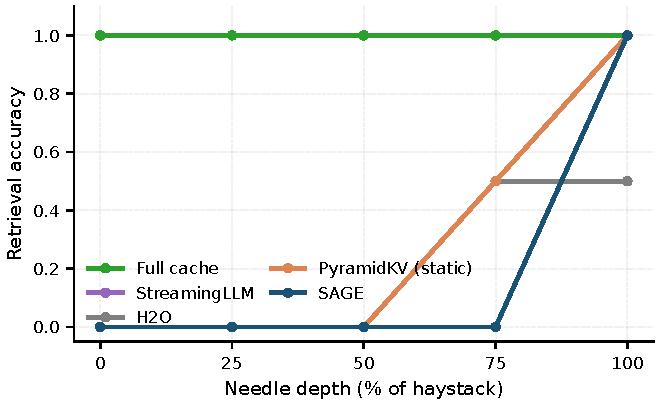
\includegraphics[width=0.78\columnwidth]{fig_needle.pdf}
\caption{Retrieval accuracy by needle depth at context 2{,}048
(Qwen2.5-0.5B-Instruct, $\rho=0.2$, matched entries). Full cache solves
the task at every depth; every history-only eviction policy loses
mid-context needles, and what survives is exactly what the retention
diagnostic says is still in the cache.}
\label{fig:needle}
\end{figure}

Table~\ref{tab:needle} and Figure~\ref{fig:needle} report retrieval; the
pattern is sharp and, we argue, under-reported in the literature.
\emph{Full cache solves the task everywhere} (accuracy 1.00 at every
depth, both lengths)---the model is not the bottleneck. Under any
history-only eviction policy at $20\%$ budget, early and mid-context
needles are lost (accuracy 0.00 at depths 0--50\% for every method,
including \sage{}), because the needle is barely attended during prefill
and scores rank it low; the question arrives only afterwards. Retention
makes the failure mode measurable: at depths where answers fail, the
fraction of needle tokens still cached is 1--5\% across scoring methods.
Two positive signals survive. \sage{}'s decay keeps late-context
structure dramatically better than undecayed baselines---mean needle
retention $0.123$ versus $0.025$ for H2O ($4.9\times$), and $0.84$
versus $0.04$ at depth 100\% of the 4{,}096-token context---and this
translates into the multi-instruction probe: with three needles asked
together, \sage{} retrieves a third of the codes (the late one) while
no-decay \sage{} retrieves none (retention $0.26$ vs.\ $0.02$ at
4{,}096). StreamingLLM's pure recency also retains depth-100 needles
(retention $0.20$) but has no mechanism at all for earlier ones. These
results calibrate what decode-time eviction can and cannot do at
aggressive budgets, and directly motivate query-aware selection
\cite{li2024snapkv,tang2024quest,xiao2024duoattention} as the necessary
complement rather than a competitor; the retention diagnostic itself is
a small methodological contribution, isolating cache-content failure from
generation failure.

\subsection{RQ6: Overhead}\label{sec:exp-overhead}

Table~\ref{tab:compliance} (right columns) reports measured per-chunk
overhead on the 2-core CPU: $2.5$\,ms (GPT-2) to $6.5$\,ms (Qwen)
scoring and $1.5$--$3.1$\,ms compression for \sage{}, comparable to H2O's
$3.3$--$8.7$\,ms scoring in the same harness (the projector adds
$<0.1$\,ms at these layer counts). Auxiliary memory at the reported
scales is $\le0.39$\,MB (Table~\ref{tab:main}), scaling at 8 bytes per
retained entry plus 8 bytes per layer per step of budget state. We
report these numbers because scoring cost is exactly what
FlashAttention-based deployments must re-compute or approximate
\cite{mao2026infra}; our eager-kernel accounting is the honest upper
bound of what the method costs when scores are materialised, and the
projection itself is architecture-independent integer arithmetic.
